\chapter{Introduction}
\label{chapter:introduction}

\section{Project description}
Sand is among the most extracted natural resources in the world. It is an essential component in the production of materials used in daily life — including electronics, ceramics, and glass — as well as in key construction materials such as concrete. As global population and infrastructure needs continue to grow, the demand for sand has increased steadily, leading to extensive mining activities across the globe. \autocite{wwfRisingDemandSand}. 
In Argentina, the Lower Paraná Delta is one of these locations that has become a critical spot for sand mining. Here, dredging companies extract  sand from the riverbed and dry sand mining companies extract it from the land. Historically, the sand was used mainly for construction but in recent years, hydraulic fracking has created a new source of demand.
While the extraction of sand can be beneficial for the economic development of the area, the impacts of the sand mining on the riverbed, the biodiversity and the surrounding delta remain insufficiently understood to draw conclusions about the sustainability of this activity. 
 
The study area focuses on a critical location of the Lower Paraná river as well as the surrounding delta. As shown in Figure \ref{fig:study area}, the area of interest stretches roughly from Puerto Ibicuy to Puerto Guazú. It includes a section of the Río Ibicuy, which later bifurcates into the Paraná to form the Paraná Guazú. The total river stretch analysed in this study extends roughly 70 kilometers. Given the dredging activities on the river, the presence of ports within the study area is also annotated in the overview in Figure \ref{fig:study area}, since they serve as key points for the transport of the extracted sand. This study considers sand mining on the river as well as on land, in order to have a comparative view on the impacts on the delta.

\begin{figure}[H]
    \centering    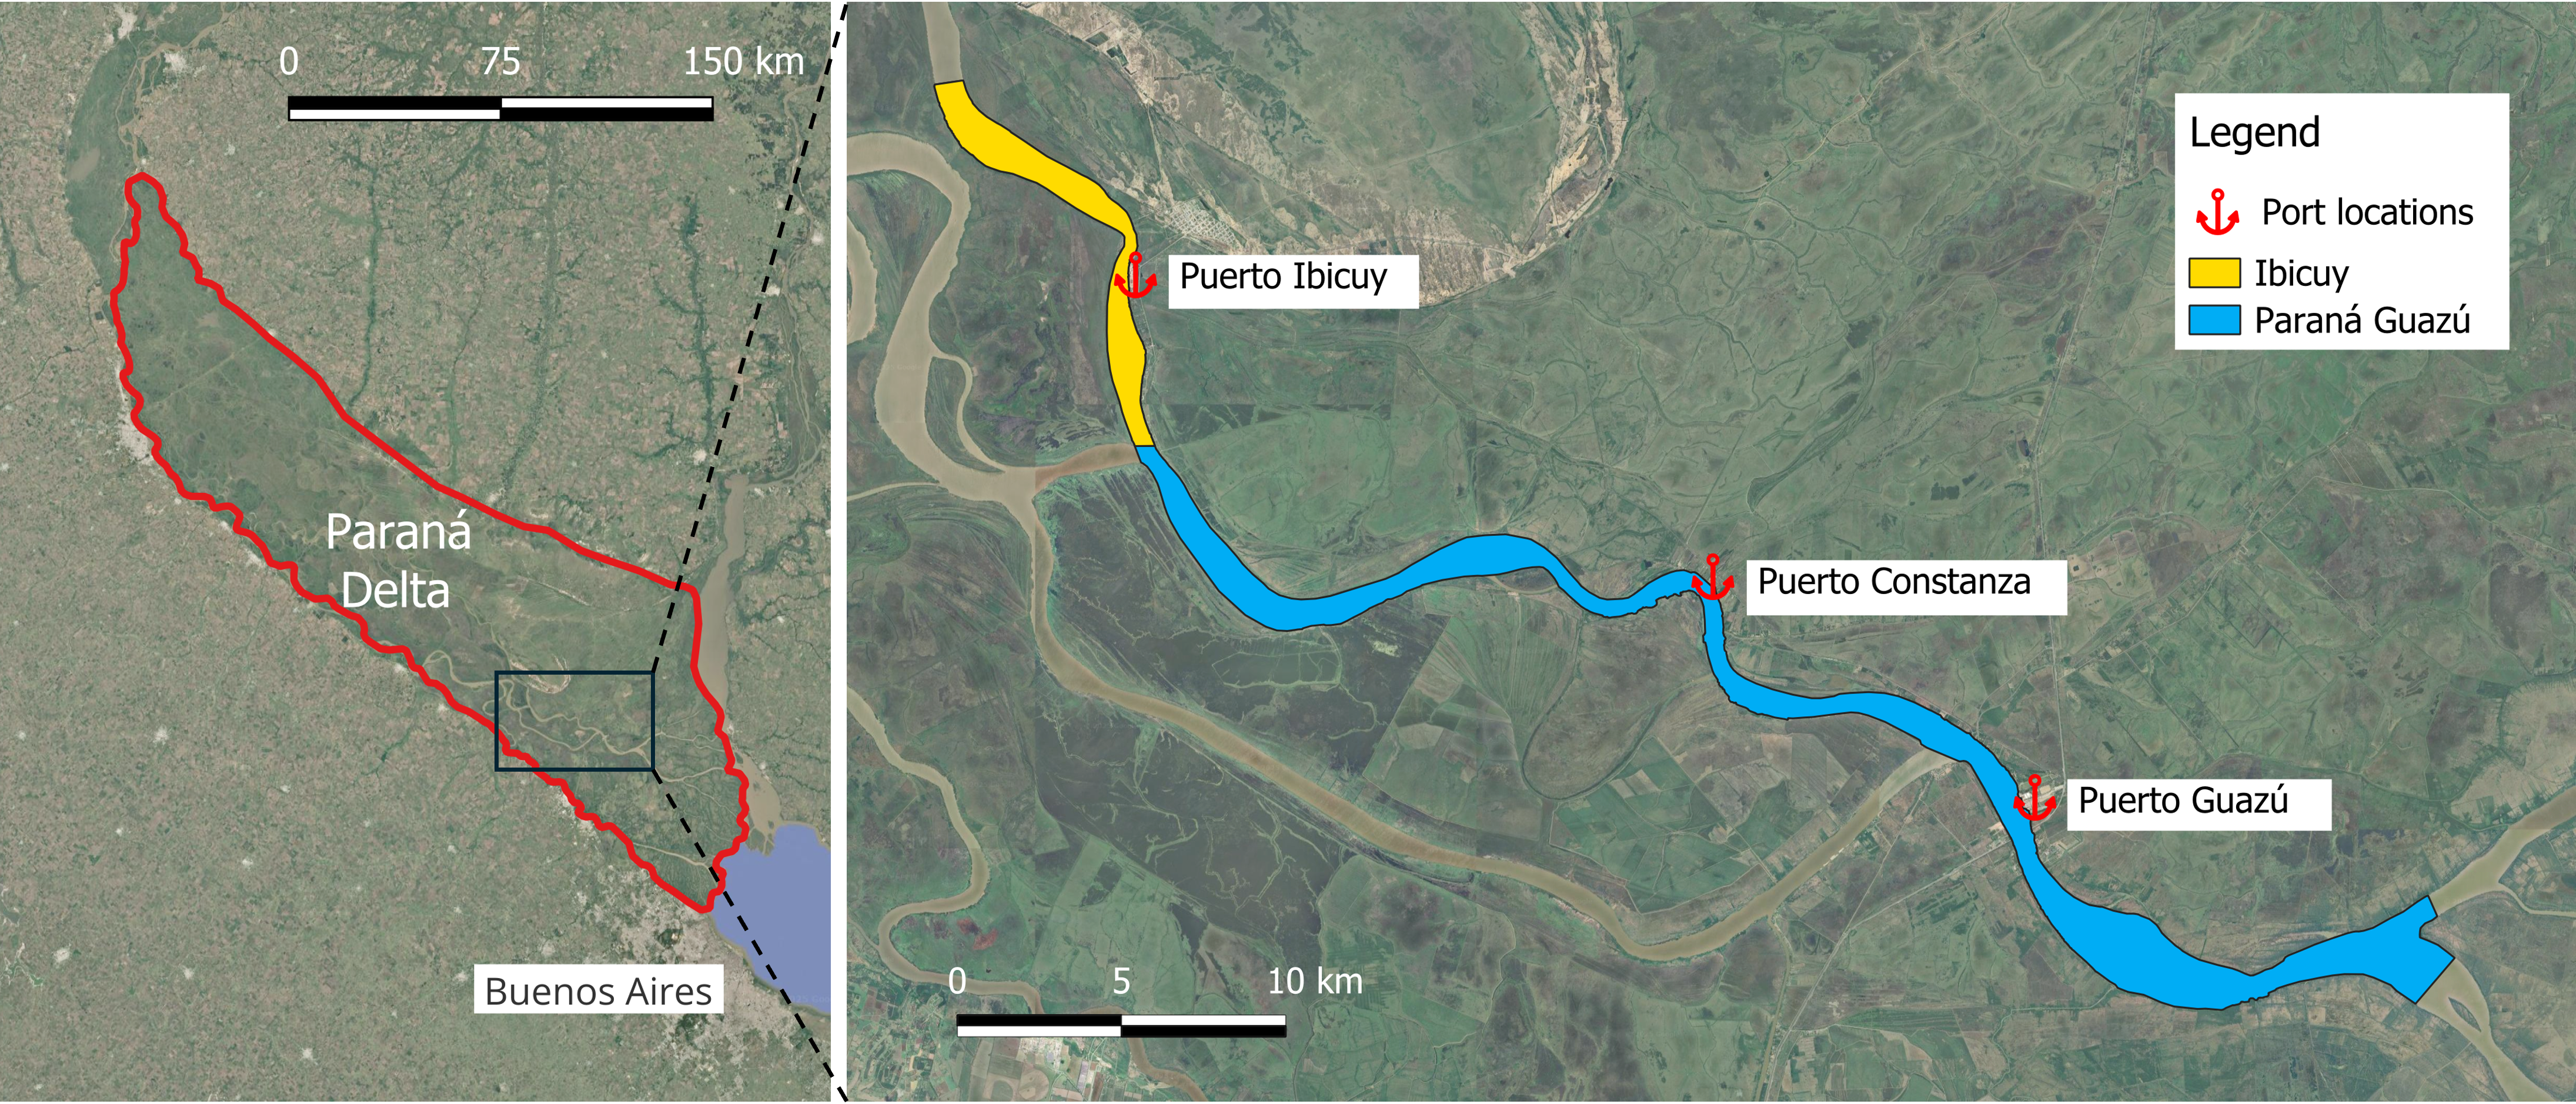
\includegraphics[width=1\linewidth]{figures/ch2/study area.png}
    \caption{Study area (\cite{googleearth2025})}
    \label{fig:study area}
\end{figure}

This project aims to determine the scale of sand mining in the Lower Paraná Delta, and to assess its diverse impacts on both the river system and surrounding land. By doing so, the study attempts to identify solutions that mitigate negative effects and find a balance that fits the needs of local communities, the existing ecosystem and the ongoing sand demand.

\section{Problem statement}

International case studies have shown the potential threat of large quantities of sand mining, such as in e.g. the Mekong delta. The negative effects of significant amounts of extracted sand and aggregates in this case can be illustrated by highly irregular bed changes over the past 10 year comparison period, stressing on an increase of mean depth of 1.3 m due to bed material losses \autocite{brunierRecentMorphologicalChanges2014}. Concluding from the Mekong case study is that sand mining is the main factor contributing to the bank erosion in the delta as well as erosion in the delta shoreline. Similar concerns about bank erosion and bank stability exist in the Paraná Delta. Furthermore, sand mining can be linked to increased morphological changes that will later impact the delta, especially in terms of sediment supply and coastal erosion.

This example is supported by a study on environmental impacts on the river due to sand mining. It states that if sediment is removed faster than it can be replenished by natural transport processes, i.e. the river has a negative sediment balance, the system may experience the following effects due to the imbalance: channel deepening, bank erosion, and changes in flow patterns \autocite{rentierEnvironmentalImpactsRiver2022}. All of these changes can have considerable consequences for navigation, infrastructure stability, aquatic habitats, and flood risk. 

Considering the hypothesis that there may be an increasing trend of dredging activities, the hydrodynamic regime of the river and the morphology of the delta may be at risk. Extracting large amounts of sand from the Lower Paraná delta can thus affect the river's natural sediment balance. Therefore, to fully grasp the extent of these impacts, it is necessary to quantify the amounts extracted, and then compare the extraction rates with the river’s natural sediment transport capacity. Without a clear assessment of the situation, the long-term sustainability of the delta and the communities and industries dependent on it remains uncertain.

\section{Objectives}

% \subsection{Project strategy}
% \subsection{Methods}
% \subsection{Multidisciplinary approach}
% \subsection{Methodology}
 
The comparative studies discussed before show that continued sand mining can cause irreversible damage to the ecological and socioeconomic environment.
Therefore, it is suggested to study the evolution of sand extraction in the Lower Paraná delta and its potential projections and implications. Specifically, an answer to the following research question is sought:

\textit{What are the morphological and socioeconomic effects of sand extraction in the Lower Paraná delta and how can these be managed to secure a sustainable future?}

In addition, a number of sub-questions are formulated to guide the reasoning of this report. The project aims to integrate perspectives from multiple disciplines and present the results in a coherent manner.

\begin{itemize} 
    \item How much sand is extracted in the Lower Paraná delta and what are its main purposes?
    \item How can the sediment balance of the Paraná Guazú river be established and quantified?
    \item What are the characteristics of river flow patterns and hydrodynamics in the study area?
    \item What are the erosion processes in the Paraná Guazú river and how are they related to dredging activities?
    \item What drives demand for sand from the Lower Paraná delta?
    \item How do the effects of river sand mining in the Lower Paraná delta differ from the effects of dry sand mining?
    \item Which structural and nature-based mitigation strategies can be proposed to reduce negative impacts?
\end{itemize}

\section{Multidisciplinary approach}
The aim of this report is to present a comprehensive assessment of the sustainability of sand mining in the Paraná Guazú. To address the complex study, this report will adopt a multidisciplinary approach, integrating experience from the fields of hydraulic, geotechnical, and structural engineering.
Accordingly, the impacts of sand mining are examined from several perspectives. The activities that represent the different disciples are as follows:

\begin{itemize}
    \item Hydraulic engineering: 
    Processing available hydrodynamic and sediment data, in order to establish a sediment balance for the Paraná Guazú.
    Understanding the river flow in the region of interest using a hydrodynamic model through the use of Delft3D software. Furthermore, tidal effects are evaluated, as well as wave interactions and effects on the bank erosion and delta. 
    
    \item Geotechnical engineering: 
    Investigation of the dry sand mining activities and the geological/geotechnical characteristics that drive the demand for sand from the region. Finally, identify possible Nature-based mitigation measures for the dry sand mining practices.
    
    \item Structural engineering: Consider different structural solutions for bank erosion and come up with a 2D-design for the most feasible one.
\end{itemize}

The interface of the disciplines is essential to have a general understanding of the problem at hand. Therefore, several actions will be tackled using advice from different disciplines. For example, structural solutions for bank erosion can only be suggested when a careful assessment of the water levels is made by hydraulic engineers, and an evaluation of the soil composition is studied by geotechnical engineers. In addition, measurements will be carried out by every profession, in which discussion is important to connect the disciplines.


\section{Report outline}
\label{section: report outline}
This section describes the structure of the report. Chapter 2 provides the background study, outlining the context of the problem and supporting later findings with theoretical foundations. Chapter 3 explains the methodology, detailing the data collection process and measurement techniques. Chapter 4 presents a stakeholder analysis, identifying the key parties involved in sand extraction activities and the interview results. Chapter 5 focuses on the sand extraction in the designated area, linking the wet and dry sand mining to the project. Chapter 6 presents an analysis performed on hydrodynamic and sediment data, gathered both from existing data sets and field work measurements. The findings of this chapter are later used in Chapter 7 for a Delft3D model, that serves to reflect the hydrodynamic regime of the study area. Building on these findings, Chapter 8 proposes mitigation strategies to address the identified impacts. Finally, Chapters 9 and 10 conclude the report with a discussion and conclusion, respectively.